HTBAC serves as a software tool to enable ensemble-based free energy protocols
to run adaptively and at scale. \mtnote{protocols?}\jdnote{addressed}.
% HTBAC is based on a co-design which integrates users i.e. domain experts and
% developers to elicit requirements.


% \mtnote{I am not sure I understand what this
% means. Domain experts and developers both elicit requirements? What about the
% rest of the development process? The sentence's grammar also needs
% attention}.

% The co-design process is iterative. For example, certain features become
% available during the software lifetime which in turn can be used by domain
% experts to build new algorithms that require such features.

% ---------------------------------------------------------------------------
\subsection{Requirements}

HTBAC has three primary requirements: (1) enable the scalable execution of
concurrent free energy protocols; (2) abstract the complexity of building
protocols
% \mtnote{``from'' instead of ``,''? See also comment in the
% following paragraph} 
from execution and resource management; and, (3) provide
adaptive features by modifying the task-graph, to enable protocols to run more 
efficiently during runtime.  

% (i.e., modifying the task-graph at runtime, based on
% previous tasks), to enable efficient protocols and effective resource sharing
% across and within protocols. 
% without explicit resource management requirements.

Based on the requirements of computational drug campaigns \mtnote{which
one?}\jdnote{keeping it general to campaigns} 
which requires the ability to run multiple concurrent protocols in order to 
scale the number of drug candidates or protein ligand systems, this poses 
several computational challenges. First, ensemble-based protocols that differ in 
computational requirements require execution coordination and resource 
management. Second, the setup of execution environments and data 
management should preserve efficient resource utilization. This poses many 
challenges that need to be addressed by HTBAC as well as the underlying 
management and runtime system. \jdnote{reworded this paragraph and hesitant 
to say workload management system.}

% and minimal overhead
% workload management system and the runtime system 
% (RTS) that support HTBAC.

% \mtnote{I am not sure I understand this sentence: grammar
% (``Based\ldots,this''?; and from the previous paragraph, we say that HTBAC
% abstracts the complexities of execution and resource management but here we
% focus on WMS and RTS? Are WMS and RTS components of HTBAC?} 

% The RTS has to
% provide sustainable submission and tracking of heterogeneous protocols
% i.e.\mtnote{note: ``i.e.'' cannot be place in the middle of a sentence
% without supporting punctuation} 
% protocols that differ in computational
% requirements, as well as setup of execution environments and data management
% while preserving efficient resource utilization and minimal
% overhead.\mtnote{Why this is relevant for HTBAC?}

Based on intermediate results during runtime, the control logic of the
algorithm may decide to invest additional compute resources in more
interesting simulations that can yield lower error averages, while reducing
resources for simulations that have already met an error threshold.
HTBAC thereby requires an adaptive execution strategy \mtnote{system}
\jdnote{changed from adaptive RTS to adaptive execution strategy} that enables 
adaptive algorithms to maximize computational efficiency.\mtnote{Seeing that we 
are speaking about requirements, does it make sense here to mention a RTS? RTS 
are an implementation detail: for example, we could design HTBAC as an 
end-to-end solution for a specific machine and still match the set of 
requirements we have reported in this subsection. Note also that we introduce 
RTS above but use ``runtime system'' again here.}\jdnote{I've removed all 
mention of workload management system and RTS and kept generality} 

Usability plays an important role in the development of HTBAC, in order to
provide a flexible interface which enables users to easily scale the number
of drug candidates and quickly prototype existing and novel free energy
protocols. Included in usability is the abstraction of adaptive features, to 
enable the user to design protocols that utilize adaptive functionality in order
to leverage intermediate results.

% ---------------------------------------------------------------------------
\subsection{Architecture}

% \subsubsection{Application Model}

We model an application in HTBAC\mtnote{what is an ``application of HTBAC''?
`In' (instead of `of') HTBAC?}\jdnote{addressed} using the following user-facing 
constructs:

\begin{itemize}
  \item \textbf{Protocol:} A generic abstraction of a free energy protocol
  such as ESMACS or TIES.
  \item \textbf{Simulation:} Simulation parameters that supply additional
  information for each protocol instance.
  \item \textbf{Runner:} Cyber-infrastructure resource abstraction for the
  application.\mtnote{``resource abstraction of the application''? Resources
  for the application?}\jdnote{addressed}
\end{itemize}

The \textbf{Protocol} construct \mtnote{we used `construct' before, as a synonym
of abstraction}\jdnote{I've removed any reference to object-orientation and kept
everything to construct in design but in implementation it changes to 
components} enables multiple instantiations of protocol types. 
The \textbf{Simulation} construct \mtnote{we used `construct' 
before, as a synonym of abstraction} specifies simulation parameters that shape 
each protocol. The \textbf{Runner} construct provides the functionality to 
specify the resource requirements and duration to execute the application.

% \subsubsection{Architecture}

HTBAC rests between the domain scientist and the cyber-infrastructure, 
abstracting the complexity of encoding end-to-end protocols and the resource and 
execution management. The Runner initializes HTBAC and holds the global state of 
the application, submits protocols and communicates with the ensemble management 
system that handles the dependencies of the protocols, and acquires resources 
via a runtime system. 


%  -----------------------------------------------------------------------------


% Protocols differ only 
% by their individual analysis step which typically follows production simulation 
% and by the computational requirements, 


% see figure X for a visual representation of
% the ESMACS and TIES workflows \mtnote{grammar. I am not able to follow the
% sentence}.


% Moreover the
% \textbf{Simulation} class provides the granularity to specify individual
% parameters per replica, including the number of cores per replica, MD
% execution kernel and the length of each simulation step.\mtnote{This might be
% seen more as a description of the implementation of HTBAC instead of its
% design}\jdnote{moved this to TIES description of implementation}

% Note that some protocols require additional information. For example, the
% TIES protocol contains additional sampling parameters or $\lambda$ windows.
% Moreover, the \textbf{Simulation} class exposes a method which enables the
% user to codify new algorithms, or modify an existing protocol such as
% specifying additional equilibration or analysis steps.\jdnote{move to 
% implementation}

% Once the protocols and simulation parameters are defined, they are passed to
% the \textbf{Runner} class where the user defines the resource requirements
% including cyber-infrastructure and duration of the application as well as
% additional flags for adaptive execution which are passed down by the
% \textbf{Runner} to the workload management and runtime systems.\mtnote{This
% seems to be mixing implementation, execution flow and architecture?}
%  -----------------------------------------------------------------------------


\mtnote{General note. It may be useful to recall the difference between
software architecture and software design. Software architecture is about the
structure of the software system, with a particular focus on modularity and
how it is rendered by components and interfaces (e.g., communication and
coordination protocols). Software design is about defining the
functionalities of each module, \textbf{showing} (i.e., arguing for) how
these functionalities address the requirements. In this context, the notion
of `class' and `method' are often regarded as implementation details, even if
object-oriented design is indeed one of the many ways to approach software
design. More in general, both architecture and design can be expressed with a
varying degree of formality and many different patterns and languages have
been and are still being developed. In this paper, we just use plain English,
informal diagrams, and a very high level overview. This approach should not
be confused with lack of precision or of scientific rigor: the goal of this
paper is to show how HTBAC architecture and design support better science in
a very specific domain, not to argue for their rigorous nature.}
\jdnote{I've modified the design to be more consistent in showing functionality
of constructs and separated architecture design from application model}


% Each replica follows the same sequence of simulation
% steps including minimization, equilibration and production simulation.\mtnote{see
% the previous comment about using `i.e.'}\jdnote{addressed}


% For TIES, where each protocol  corresponds to a single physical system. The
% TIES protocol object enables the user to select a physical system, number
% of replicas, core allocation per replica, and $\lambda$ windows to sample.
% Figure~\ref{fig:pst} provides the visual implementation of the TIES
% protocols into the PST model.

% ---------------------------------------------------------------------------
\subsection{Implementation}

% The \textbf{Protocol} construct is the main abstraction of HTBAC. 

HTBAC is a domain specific library implemented in Python. All components of 
HTBAC are implemented as objects. An application of HTBAC consists of one or 
more protocol instance(s). Each protocol models a unique protein ligand physical 
system \mtnote{see the previous comment about using `i.e.'}\jdnote{removed i.e.}. 
Each protocol follows a sequence of simulation and analysis steps and assigns 
ensemble members to execute independent simulations or analysis. An ensemble 
member that executes an independent simulation within a simulation step is 
referred to as a \textbf{replica}. Each replica simulation is assigned a 
different initial velocity, which enables simulations to begin in different 
parts of the ligand's phase space. 

We define an individual simulation or analysis as a computational \textbf{task}, 
which has a defined input, output, termination criteria and dedicated 
resources~\cite{power-of-many17}. Aggregates of tasks with dependencies that 
determine the order of their execution describe \textbf{workflows}. A workflow 
is comprised of $N_P$ instances of the P$^{th}$ protocol.\jdnote{does this 
confuse the term application with workflow?}

HTBAC uses the RADICAL-Cybertools (RCTs) which are middleware building 
blocks~\cite{review_bb_2016} that support HTBAC's workflow execution across 
diverse computing platforms~\cite{turilli2017comprehensive}. HTBAC rests on two 
primary RCT libraries, Ensemble Toolkit (EnTK) and RADICAL-Pilot (RP).

EnTK serves HTBAC as the ensemble management system that provides specific 
interfaces and execution models for ensemble-based 
applications~\cite{power-of-many17}. EnTK provides an application model that 
simplifies both the encoding and execution of scalable and adaptive free energy 
protocols that differ in computational requirements. HTBAC uses the programming 
model of EnTK to construct workflows. EnTK exposes 3 
user-facing constructs, \textbf{Task}, \textbf{Stage} and \textbf{Pipeline}. 
Reference~\cite{power-of-many17} defines these constructs as follows: a task 
contains information regarding an executable, its software environment and its 
data dependencies. A stage is a set of tasks without mutual dependencies and 
that can be executed concurrently. A pipeline is a list of stages where any 
stage $i$ can only be executed after stage $i - 1$ has been executed. Each 
pipeline can execute independently. In HTBAC, a protocol instance is encoded as 
a single pipeline, which contains stages of simulation and analysis steps. 
Replicas or analysis tasks are bundled as tasks within a stage. We show the 
implementation of two types of protocol types, ESMACS and TIES.

\subsection{ESMACS and TIES}

While ESMACS and TIES protocols compute binding affinity calculations for 
different systems and purposes, their implementation in HTBAC have a similar 
pattern that consists of simulations steps, followed by one or more analysis 
step(s). In this paper, we focus on the default sequence of simulation steps 
which consist of minimization, initial equilibration, secondary equilibration, 
and production MD simulation. Designers of free energy protocols are not bound 
by this sequence and can utilize the Protocol component to provide an
alternative sequence. ESMACS contains 25 replicas per simulation step. TIES 
contains a $\lambda$ sampling parameter which generates 5 replicas per 
$\lambda$ window. In this paper, we implement TIES with 13 $\lambda$ windows to 
spawn a total of 65 replicas in each simulation step. 
Figure~\ref{ties_esmacs_application} demonstrates the implementation of the 
ESMACS and TIES protocols. 

\begin{figure}
  \centering
  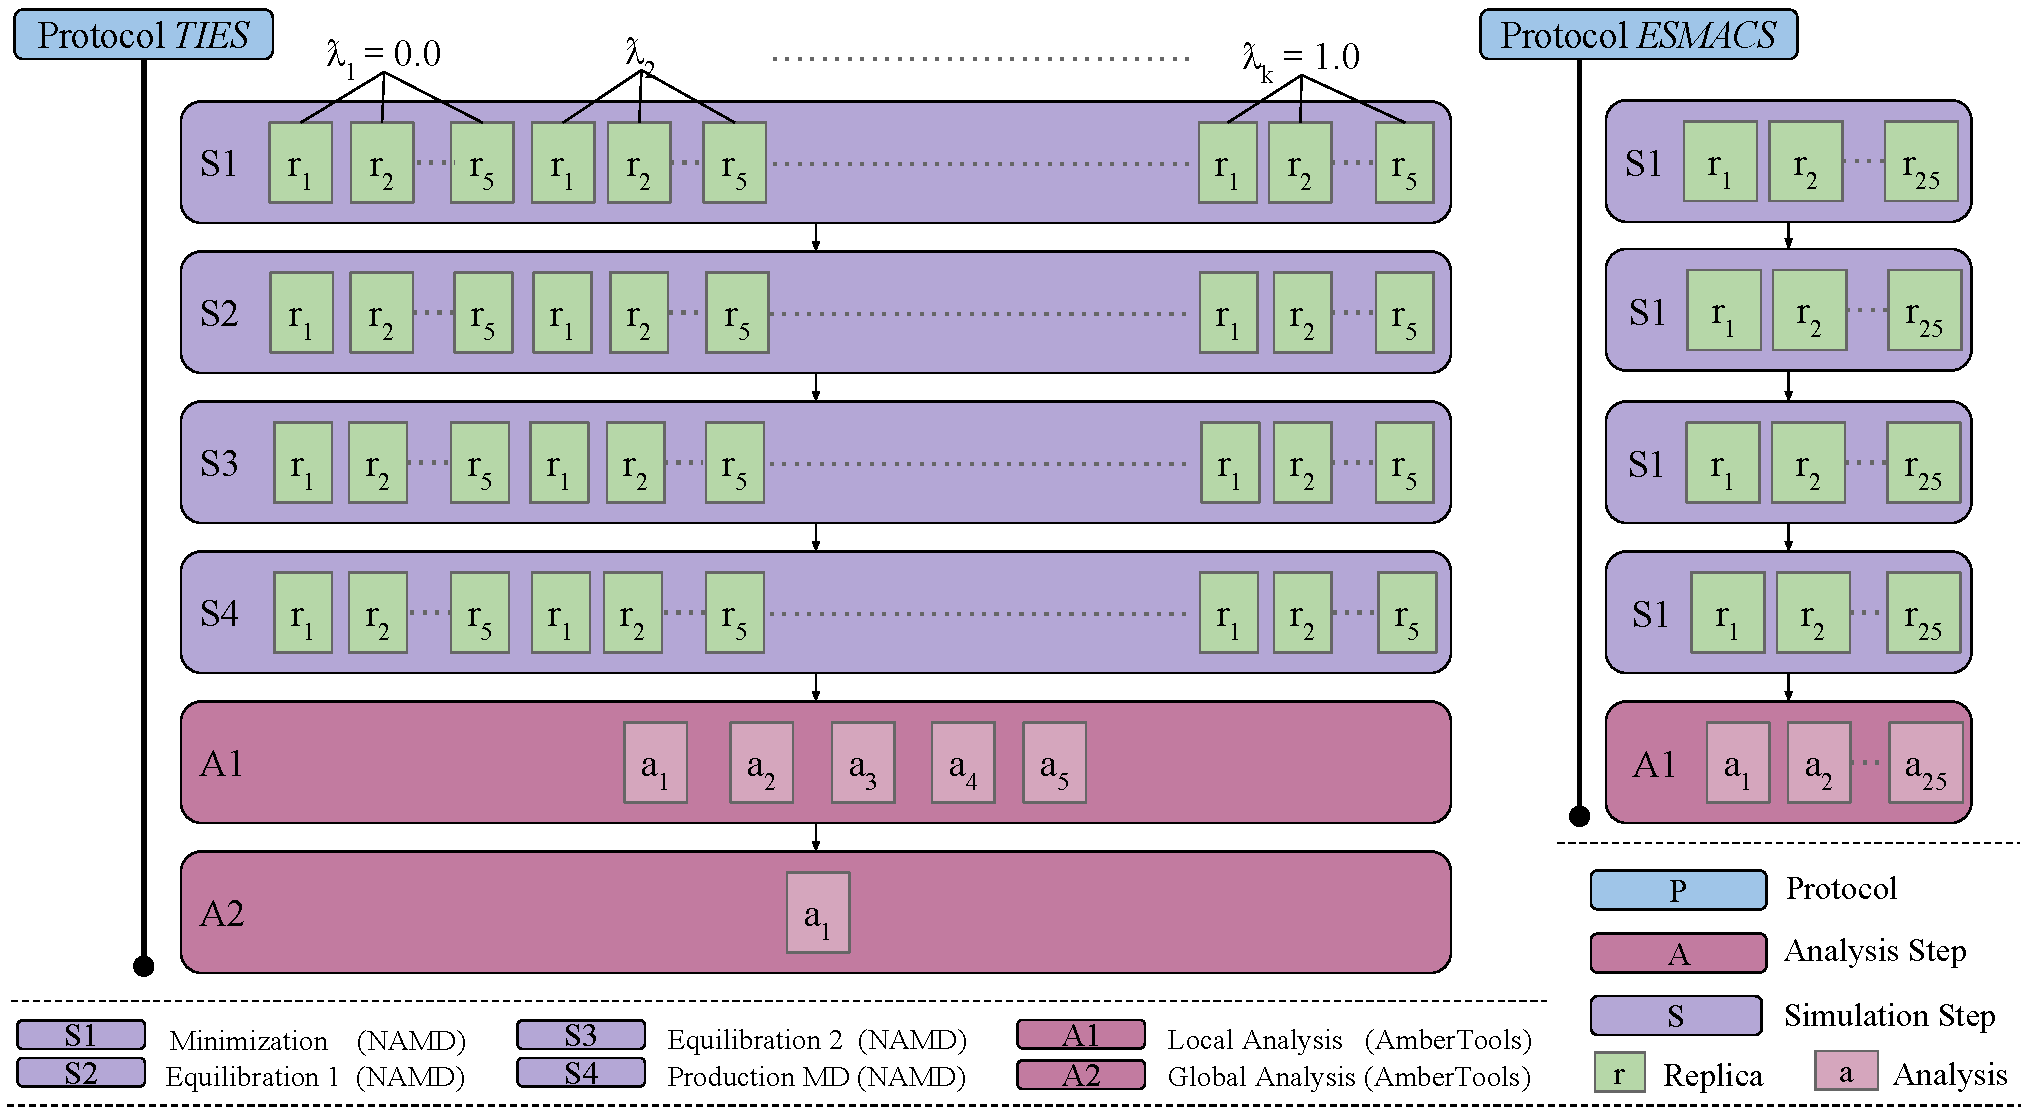
\includegraphics[width=\columnwidth]{figures/ties_esmacs_application_model.pdf}
  \captionsetup{singlelinecheck=off}
  \caption[]{TIES and ESMACS protocols consist of simulations steps followed 
  by analysis step(s). All replicas within a simulation step are assigned the 
  following simulation timesteps, for 6 nanoseconds simulation duration.
     \begin{itemize}[label={--}]
      \item $S1$ : 1000
      \item $S2$ : 30,000
      \item $S3$ : 800,000
      \item $S4$ : 2,000,000 
    \end{itemize}
  }
\label{fig:ties_esmacs_application}
\end{figure}

The analysis step(s) vary according to each protocol. ESMACS contains a 
single analysis step with 25 tasks that computes the MMPBSA with respect to each 
replica.\jdnote{MMPBSA needs to be defined in feprotocol} TIES contains two 
analysis steps. The first step is a local analysis containing 5 tasks that 
aggregate the simulation results of each replica using the Hamiltonian 
derivative calculation. This is followed by a global analysis stage that 
contains a single task to calculate the thermodynamic integration across 
replicas. 

% In HTBAC, each replica is encoded as a pipeline, which contains stages of 
% simulation steps. Each stage contains a single task which performs a
% simulation. Each protocol consists of an aggregate of replicas, or independent 
% pipelines. 

\subsection{Intra-protocol Adaptivity} 

% Protocols that have the ability to 
% The flexibility at the protocol component enables the user to modify the 
% simulation steps.

Given a protocol type such as ESMACS or TIES the user can create an adaptive or
nonadaptive workflow. The nonadaptive workflow specifies all its requirements 
prior to execution. The adaptive workflow provides partial requirements but 
learns the remaining requirements during execution. 

Intra-protocol adaptivity is a type of adaptive workflow that relies on the 
intermediate results \textit{within} a protocol instance to define the next set 
of requirements. We demonstrate the implementation of an intra-protocol adaptive 
workflow using the TIES protocol. As indicated in section~\ref{science-drivers}, 
the optimal positions of the $\lambda$ windows are not known \textit{a priori}. 
Therefore the number of simulations and their descriptions, which are 
dictated the $\lambda$ windows parameter, cannot be pre-specified in the 
workflow. 

Instead, we construct an adaptive workflow for TIES as an iterative pipeline in 
two stages: a simulation step and analysis which determines optimal 
placement of further simulations, as shown in Figure~\ref{adaptive_ties}. We 
initialize the workflow with $y$ evenly spaced $\lambda$ windows, which 
generates $y \times n$ initial replicas. After the first pass of simulations, 
the analysis operates on the simulation results to determine 
the next placement of $\lambda$ windows and generates a new set of simulation 
configurations for the upcoming iterations. Each simulation step within an 
iteration executes for a single nanosecond simulation duration. The analysis 
consists of a single task that computes the adaptive quadratures 
calculations as defined in section~\ref{science-drivers} which decides whether 
to spawn additional $\lambda$ windows \textit{in between} existing windows. This 
enables continuous execution of existing simulations and beginning of new 
simulations. The workflow is executed iteratively until the total simulation 
duration, as defined by the user, determines termination. 

\begin{figure}
  \centering
  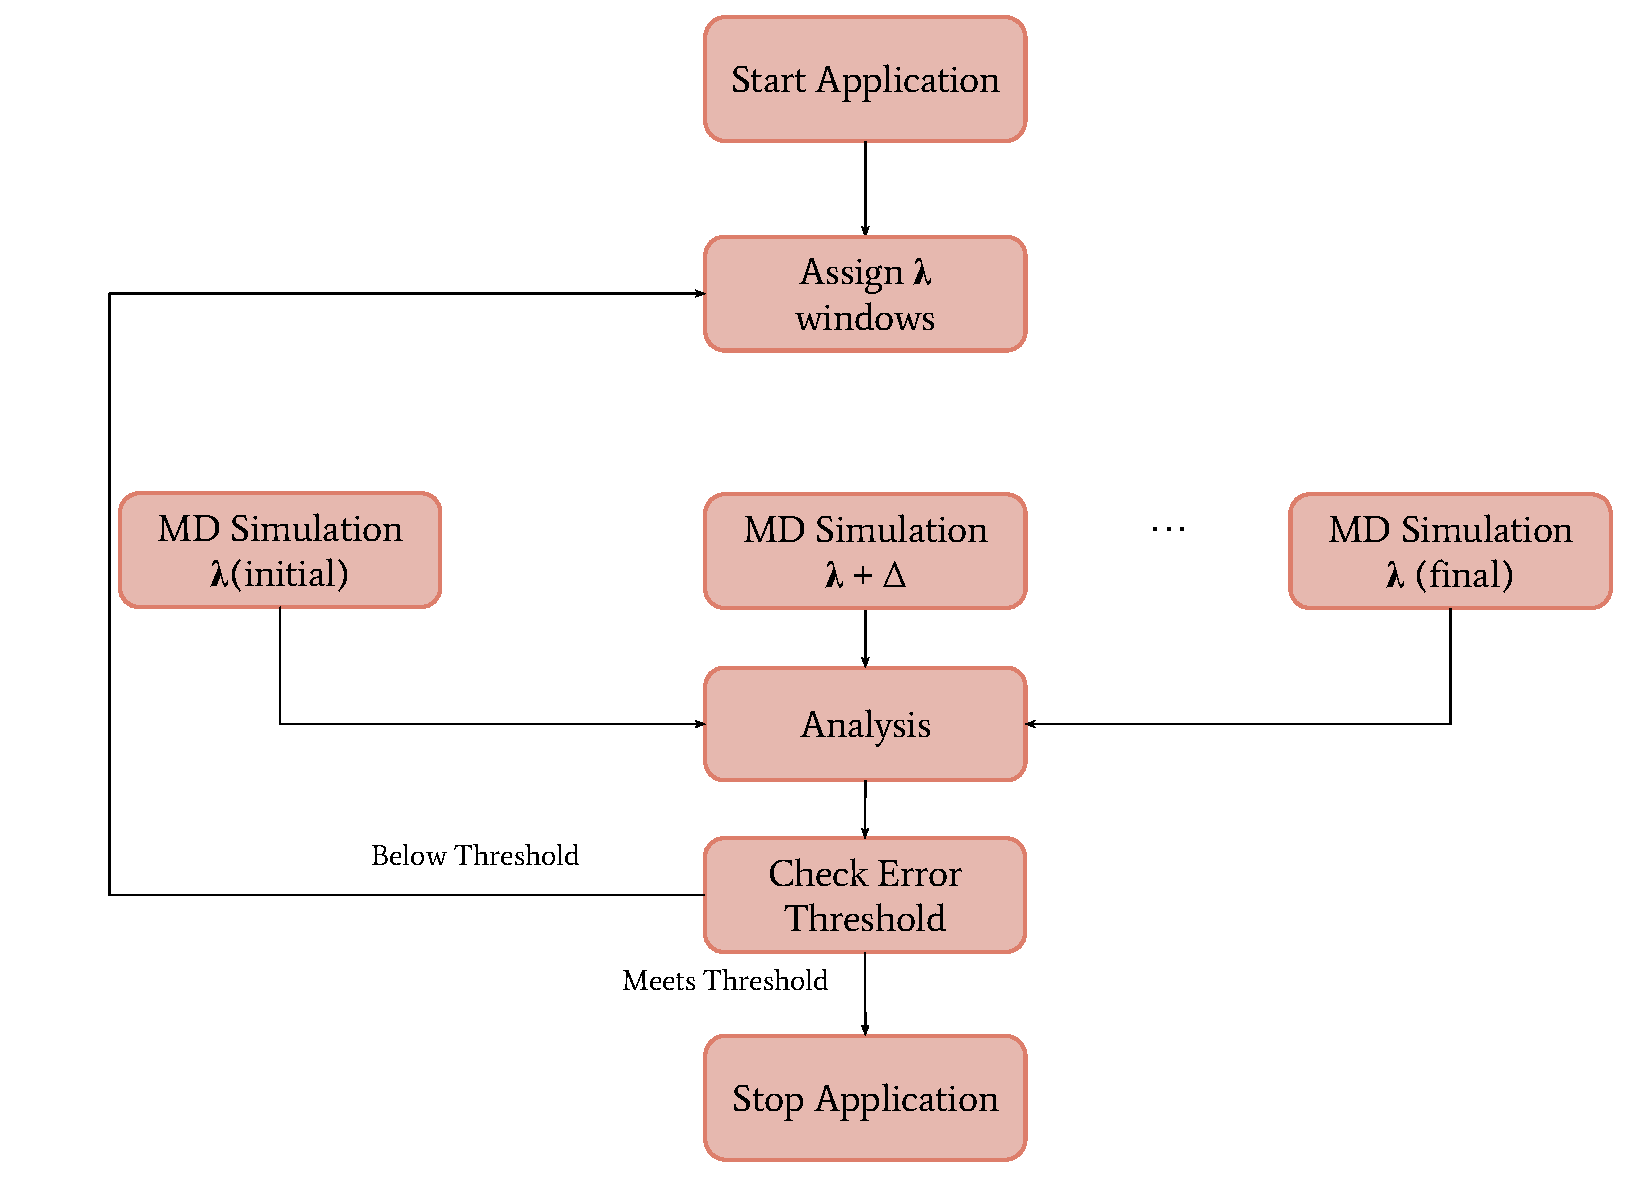
\includegraphics[width=\columnwidth]{figures/adaptive_TIES_workflow_diagram.pdf}
  \caption{Adaptive workflow of TIES consisting of multiple concurrent and
  independent simulations. The analysis (adaptive quadratures) operates on 
  a snapshot of the current simulations for each $\lambda$ window, and decides 
  if the critical threshold is reached, else current simulations continue 
  executing and new simulations are spawned based on additional $\lambda$ 
  values.}
\label{fig:adaptive_ties}
\end{figure}

\subsection{Execution Model}

Once an adaptive or static workflow is described in HTBAC, 
\mtnote{the previous paragraph does not
mention workflow(s) so this surprises and confuses the reader. Note that this
is a byproduct of commenting out part of the text where a connection between
protocol and workflow was explicitly established}

\jdnote{provided earlier 
definition of workflows}, the Runner component tags each protocol instance with 
a unique ID and converts protocols into EnTK pipelines. 
% EnTK abstracts the complexity of execution and resource management. 
Pipelines are submitted to EnTK's \textbf{Application Manager} which sets up 
multiple processes, threads and a message queue for communication. EnTK 
identifies tasks which have satisfied dependencies and can be executed 
concurrently. EnTK's \textbf{Execution Manager} uses its underlying runtime 
system RADICAL-Pilot (RP) to execute the tasks on specific target resources. 
EnTK converts the set of pipelines into a set of tasks---called compute unit 
descriptions---and submits them to RP \mtnote{Is RP defined?}\jdnote{It is now}.

The Runner component of HTBAC describes the computational requirements of the 
workflow including walltime, cores, queue, and user credentials 
\mtnote{of what?}\jdnote{addressed} for which EnTK creates a resource request. 
EnTK converts this resource request into a pilot that RP submits to an HPC 
machine. Once the pilot becomes active, it pulls compute unit descriptions in 
bulk from a database, executing them on the pilot 
resources~\cite{merzky2015radical}. 

Figure~\ref{} shows a visual block diagram representation
\mtnote{`visual block diagram representation' seems unclear to me. Should we
just have an architecture diagram here?} of HTBAC and the underlying building
blocks.\jdnote{adding architecture diagram -- in draft currently}

\subsection{Adaptive Execution Model}

Support for intra-protocol adaptive workflows requires an adaptive execution 
strategy. We leverage the adaptive capabilities provided by 
EnTK~\cite{adaptivebiomolecular} to raise the level of adaptive features 
abstraction in HTBAC. 

intra-protocol adaptivity schema requires the 
redistribution of resources to account for additional simulations generated 
during runtime. 

% As demonstrated by the requirements of the TIES intra-protocol 
% adaptivity schema, the runtime system that provisions resources to support 
% execution of concurrent simulations will need to redistribute resources in order 
% to support concurrent execution of both existing and new simulations. 

Using the protocol, runner, simulation components, users express the initial 
protocol configuration and resource requirements. The user also provides the 
analysis script that is required to generate conditions of new simulations. 

% The workflow method exposed by
% the protocol component enables granularity in creating multiple ``shorter" 
% protocols. 

The runner maintains the state of the submitted protocol by tagging each 
protocol instance with a unique ID. This enables the runner to keep track of
protocol instances that require additional simulations. 
% The protocol component 
% contains a post-execution property that invokes the application once the protocol 
% terminates. In HTBAC, the 

Once simulations have executed, a post-execution property of the protocol object
performs a write operation of the simulation results. After the initial protocol 
executes, the control logic returns back to the main script where the user has 
already pre-specified a function that computes the next placement of simulations 
based on the output generated by the protocol. The choice of this strategy is to 
account for various functionalities that are specific to the requirements of the 
user. The protocol component contains a parameter that accepts new simulation 
conditions and builds a new workflow that extends the current protocol by 
incorporating new simulations.

As the number of simulations grows during runtime, the ratio of cores-to-task 
fluctuates. The runner redistributes an even share of the total requested cores 
to each simulation. This strategy was based on the assumption that the runtime 
system does not provide dynamic pilots, where additional resources can be 
submitted to the batch system. In addition, by design of ensemble-based free
energy protocols, all simulations require the same resources. 

The \textbf{Application Manager} in EnTK signals RP to 
bypass termination of the pilot and instead keep the session alive, as long as 
additional tasks are submitted within provisional walltime. \mtnote{I tried to 
fix a bit the paragraph but it still difficult to read and understand.}
\jdnote{a lot has changed in this subsection...}


% Spawning of new task contribute to task count adaptivity and task attribute
% adaptivity. Using EnTK, HTBAC creates the necessary set of new tasks.






% In section~\ref{sec:science-drivers}, we described a particular type of
% adaptivity within TIES that would enable the simulation \mtnote{which one? Or
% should this be `a simulation' or `simulations'?} to reach convergence
% earlier. Figure~\ref{fig:adaptive_ties} illustrates the adaptive workflow of
% TIES (change $\lambda$ step size as $\delta$ \mtnote{is this a comment?
% Please clearly identify comments in the text.}). Adaptive execution requires
% changes to the task graph during runtime, a capability supported by the RCT
% runtime layers~\cite{power-of-many17}.

% The TIES adaptive workflow decides, postmortem \mtnote{no dash}, about the
% placement of new $\lambda$ windows for the next set of simulations. In turn,
% the workflow makes runtime decisions about the number of tasks in the task
% graph. This type of adaptivity in the workflow requires as \mtnote{as what?
% Requires capabilities to count tasks and changing the attribute of tasks
% depending on \ldots?} task-count and task-attribute
% adaptivity~\cite{adaptivebiomolecular}.

% HTBAC monitors the output of the completed tasks during runtime, and
% redefines the existing workflow by adding more $\lambda$ windows \mtnote{as
% required? The sentence appears to be incomplete}. A boolean results generated
% at the end of a pipeline defines a criteria of whether or not
% \mtnote{when using `whether' the `or not' is implied} to spawn additional
% tasks. 



% For users to design an 
% adaptive workflow requires the flexibility and granularity to enhance specific 
% parts of the workflow to act upon runtime decisions. 

% Within a protocol, there may
% be a case for hybrid workflows. Certain steps in the protocol may be completely 
% specified while others require stopping the simulations to perform an 
% evaluation that aids in deciding the continued set of requirements. 


% In HTBAC, the protocol component allows the user to decompose a single
% protocol instance into multiple protocols that execute shorter simulations.

% When describing the application, the user can directly specify between 
% sub-protocols that analyze results of the most recent snapshot of simulations, 
% and exchange this information with the next sub-protocol. 

% In HTBAC, the application terminates once the control logic returns to the user
% after executing all protocols. The segmented sub-protocols allow for more 
% control between executions. 



% TIES 
% -------------------------------------------------------------------------------

% In EnTK, a Pipeline is created for each unique combination of the following parameters:
% system, replica, and thermodynamic state i.e. $\lambda$ window in the case of
% TIES~\ref{fig:ties_workflow} \mtnote{This paragraph overlaps in scope with
% the last part of the previous paragraph. This results in repetition and
% confusion for the reader. Also, note that punctuation is missing, including
% the one closing the sentence.}
% -------------------------------------------------------------------------------

% A protocol 
% defines a % simulation 
% pipeline composed of an ordered sequence of simulation steps. In
% ensemble-based, free energy protocols such as ESMACS or TIES, these
% pipelines are replicated, where replicas differ by their parameter
% configurations. For example, in ESMACS and TIES, replicas only differ by initial
% velocities, which are assigned randomly by the MD engine at the start of
% execution. By nature of ensemble applications, each replica within a protocol
% can execute its pipeline independently.


% Sets of tasks with dependencies that determine the order of their execution
% are usually referred to as “workflows”.

% In section \ref{sec:science-drivers}, we described two examples of
% ensemble-based protocols for computing binding affinities.



% A computational
% \textbf{task} represents an independent simulation. Aggregates of tasks
% create \textbf{workflows} 




% \begin{figure}
%   \centering
%   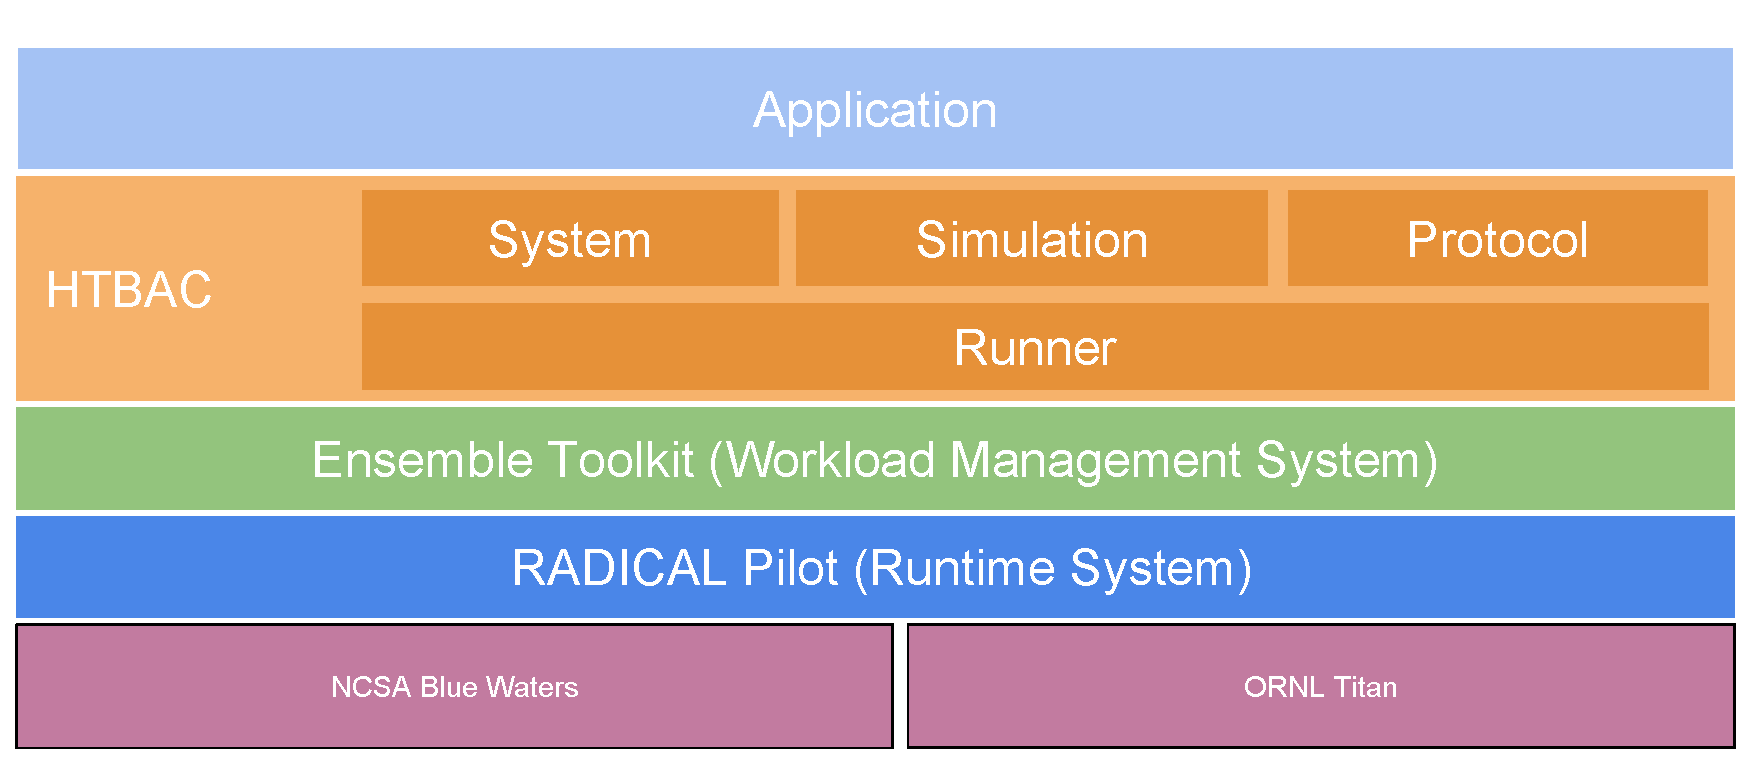
\includegraphics[width=\columnwidth]{figures/building_blocks.pdf}
%   \caption{Layered architecture of HTBAC, EnTK, and RP. The HTBAC API
%   exposes the Protocol component. Current protocols supporting the use cases
%   include ESMACS and TIES. EnTK serves as the workload execution system.
%   RADICAL-Pilot serves as the runtime system.}
% \label{fig:blockdiagram}
% \end{figure}




% ---------------------------------------------------------------------------
% \subsubsection{Workload Management and Runtime System}

% EnTK simplifies the process of creating ensemble-based applications with
% complex coordination and communication requirements. The EnTK API exposes the
% PST model which consists of three components\mtnote{I am not sure these are
% components. There is the risk to consider them architectural elements when
% they are not}: \textbf{Pipeline}, \textbf{Stage}, and \textbf{Task}. HTBAC
% promotes binding affinity \textbf{Protocols} as the user-facing construct,
% and uses the programming model defined by the Pipeline, Stage and Tasks model
% to express a specific protocol. \mtnote{The second part of this paragraph is
% inconsistent with the first: for example, see the use of PST and then
% `Pipeline, Stage and Task', or the use of protocols with capitalization
% (proper names are not plural) without differentiating them (it?) from those
% defined in EnTK via PST}

% Each HTBAC application aggregates one or more protocols. A workflow is
% comprised of $N_P$ instances of the P$^{th}$ protocol.

% each stage is a computational \textbf{task}, and the ordered aggregation of
% these stages alongside their dependencies as a
% \textbf{pipeline}~\cite{power-of-many17}.

% Sets of tasks with dependencies that determine the order of their execution
% are usually referred to as “workflows”.

% In section \ref{sec:science-drivers}, we described two examples of
% ensemble-based protocols for computing binding affinities.



% \begin{figure}
%   \centering
%   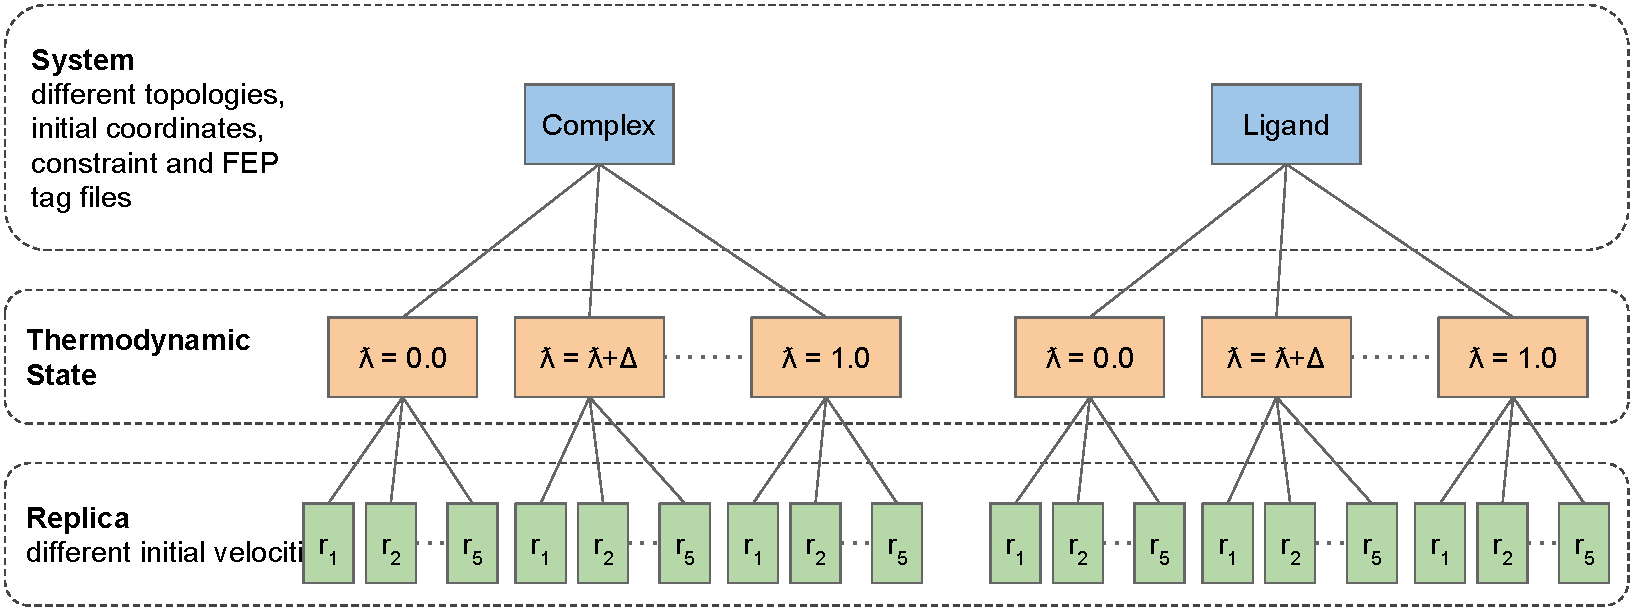
\includegraphics[width=\columnwidth]{figures/ties_workflow.pdf}
%   \caption{TIES workflow consisting a physical system, thermodynamic states
%   and replicas. Each replica is assigned a thermodynamic state. The workflow
%   is translated into an EnTK PST workflow. Construction Number of EnTK
%   Pipelines = 2 * (($\lambda$(max)/$\delta$) + 1) * 5 where $\lambda$(max) =
%   1 }
% \label{fig:ties_workflow}
% \end{figure}

  
\begin{figure}
  \centering
  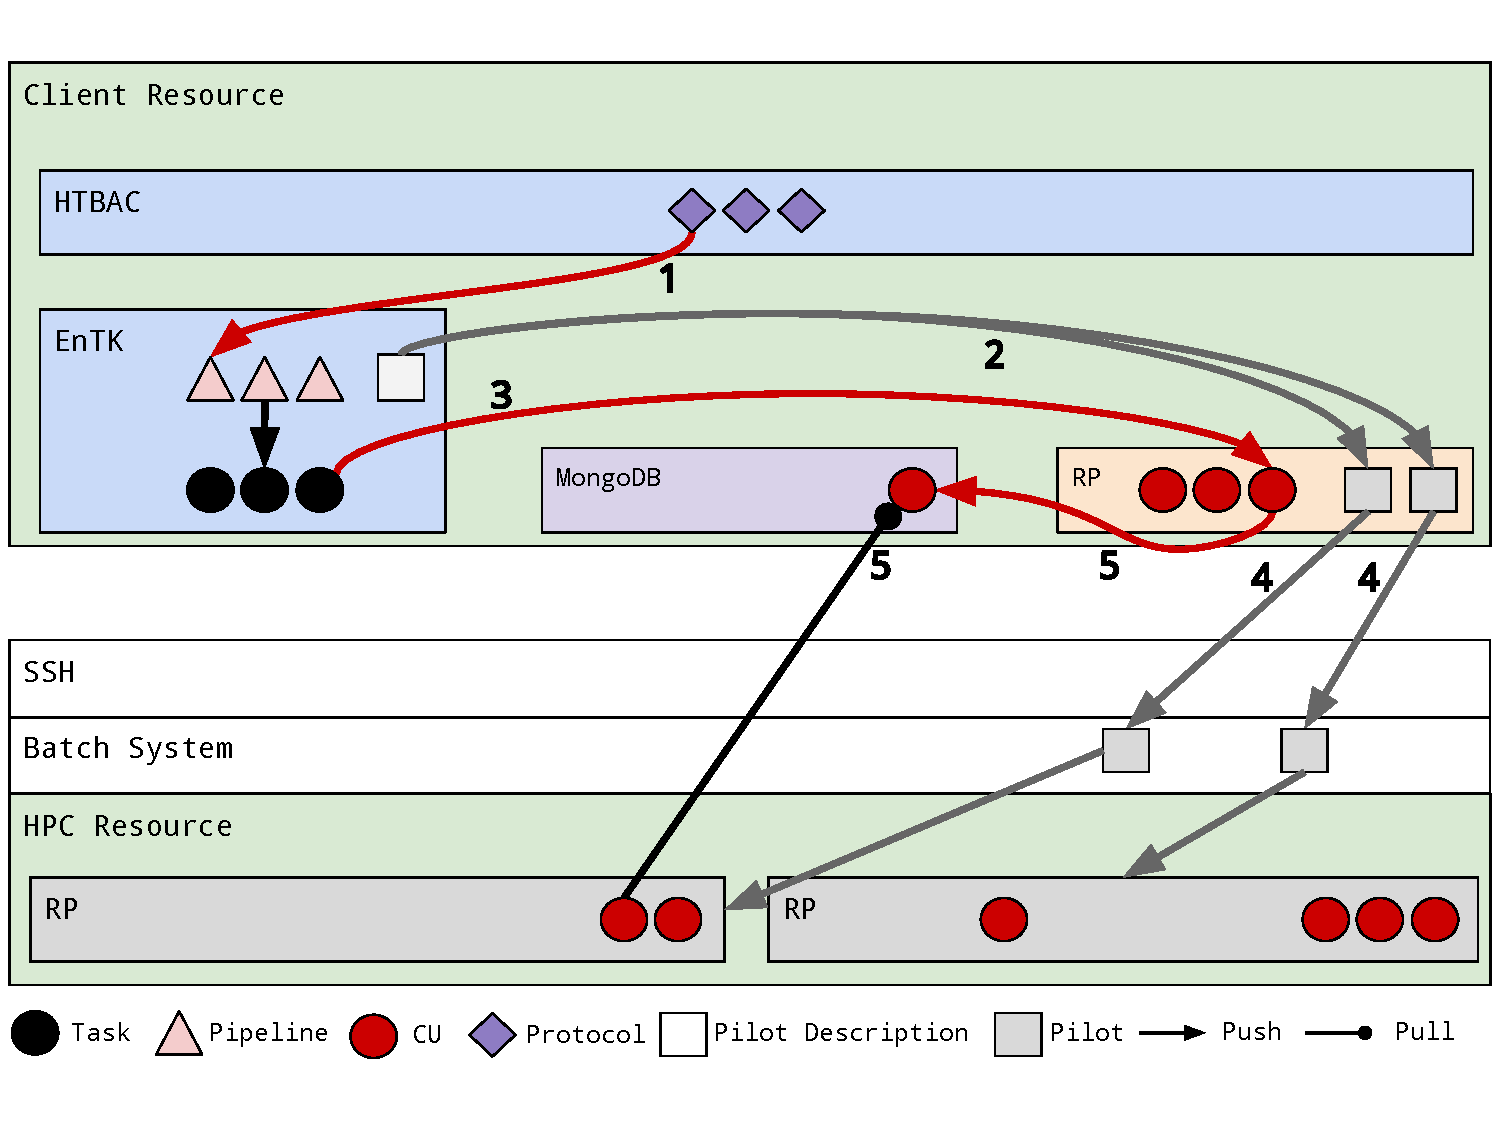
\includegraphics[width=\columnwidth]{figures/ht-bac-rp_integration.pdf}
  \caption{Ensemble Toolkit (EnTK) and RADICAL-Pilot (RP) architecture and
  execution model.\mtnote{Unreferenced figure.}}
\label{fig:integration}
\end{figure}

% Consistent with EnTK's programming model, HTBAC also uses the PST model to
% express {\bf Protocols}.

% Each protocol contains multiple stages with simulations and analysis tasks
% interspersed, in the most general case.

% programming model (that are consistent with the EnTK) to enable the user 

% HTBAC rests upon established middleware solutions~\cite{review_bb_2016},
% validated runtime abstractions~\cite{turilli2017comprehensive} for scalable
% execution, and customizes them for the computation of binding free
% energies.

% HTBAC derives many of the advantages of a lightweight, flexible domain
% specific workflow layer from its use of RADICAL-Cybertools (RCT) which are
% functionally well-defined and delineated middleware building blocks.
% RCT~\cite{review_bb_2016} are engineered to support extensible and scalable
% workflows across diverse computing platforms. The two primary RCT
% components that HTBAC depends upon are the Ensemble Toolkit (EnTK) and
% RADICAL-Pilot (RP).

% (so far, a workflow entails a maximum value of $P = 2$ and $N_P$=16, but in
% future work P will be greater $>$ 2).

% protocol, a user can scale protocol instances to study as many physical
% systems as desired.

% The specification of protocols and their parameters are passed by the user
% to the \textbf{Runner Handle} which translates the request to EnTK.

% In Section \ref{sec:related-work} we highlighted how an ensemble simulation
% approach can both aid sampling and improve uncertainty quantification for
% free energy calculations. Despite these crucial advantages, it remains
% non-trivial for field researchers to write biosimulation applications that
% involve individual protocols supporting multiple replicas, and by extension
% multiple protocols. With HTBAC, this burden is minimized by specifying the
% number of concurrent instances of the \textbf{Protocol} object. Moreover,
% the ability to generate multiple protocol instances enables the user to
% investigate a range of physical systems (i.e., drug candidates)
% concurrently.

% HTBAC allows the simple expression and concurrent execution of multiple
% distinct protocols, thereby enabling concurrent screening of drug
% candidates. HTBAC not only simplifies the expression of complex binding
% affinity protocols, but also provides hitherto unavailable capabilities,
% viz., the adaptive execution of these protocols, without any additional
% programming burden.

% Explain adaptive API and how it is passed to EnTK\mtnote{Please clearly
% identify comments in the text.}

% In turn, our adaptive execution implementation at the WMS focuses on
% supporting generality of adaptive workflows at the inter and intra-protocol
% level.

% \begin{figure}
%   \centering
%    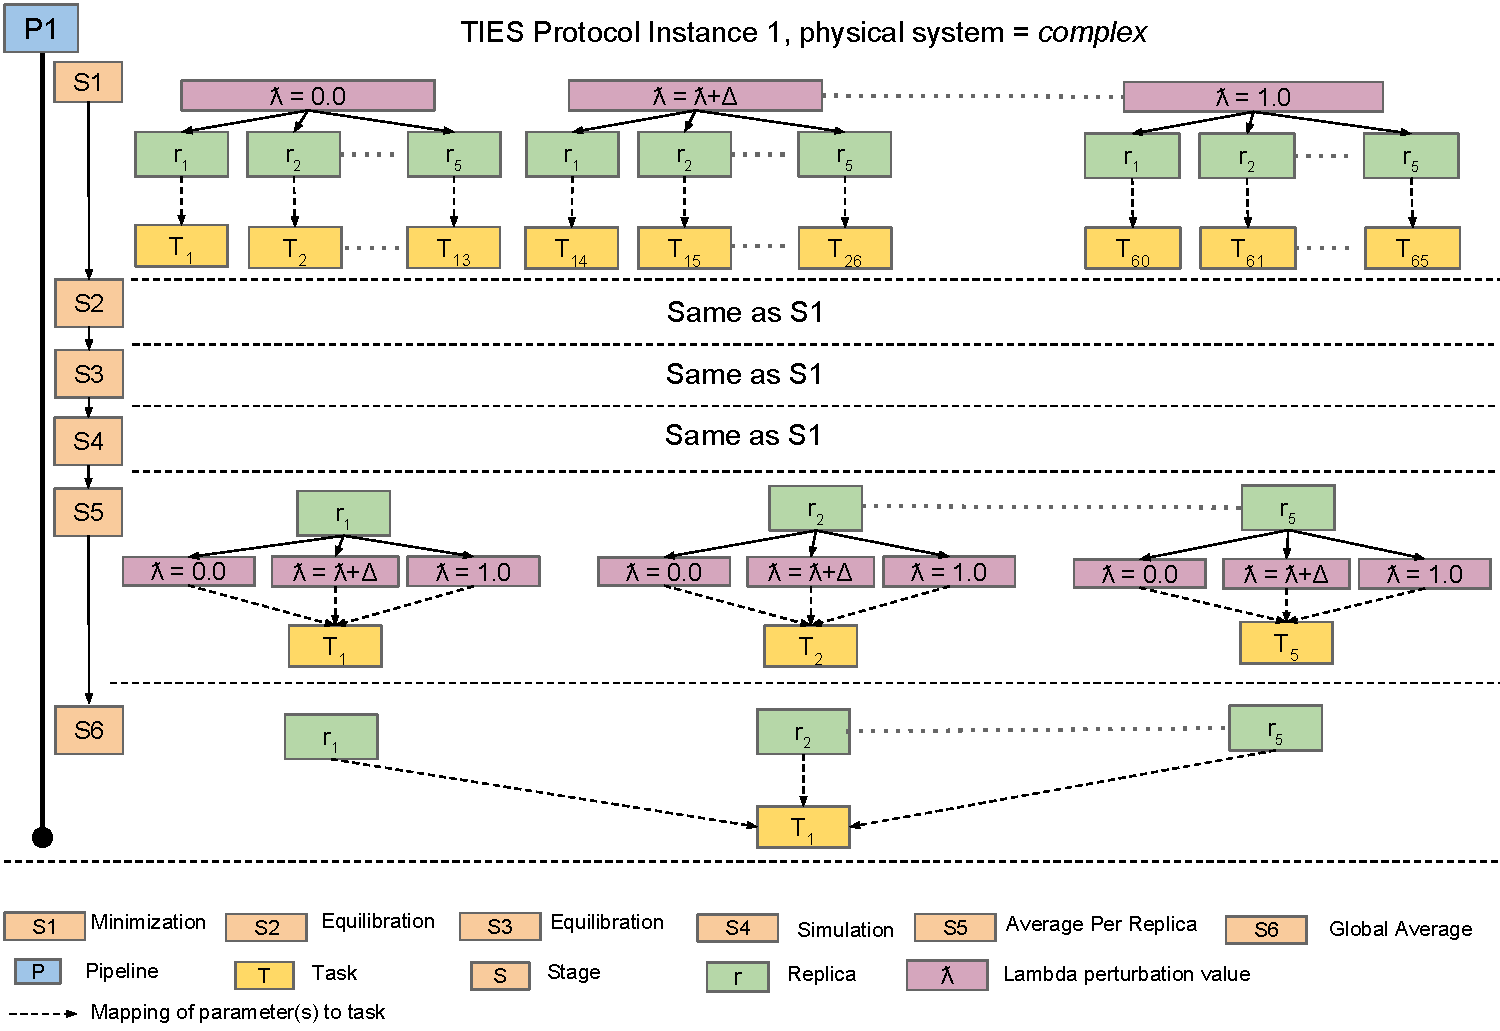
\includegraphics[width=\columnwidth]{figures/_TIES_EnTK_implementation.p
%    df}
%   \caption{TIES protocol expressed using the EnTK PST model. Each protocol
%   instance maps to a single Pipeline, comprised of Stage(s) which maintain
%   temporal order. Each Stage executes $n$ tasks, where $n$ represents the
%   number of unique lambda-replica combinations.}
% \label{fig:pst}
% \end{figure}


% \subsection{Scalability}

% Each protocol instance studies a single physical system i.e. drug
% candidate. By extension, the user is able to scale the number of concurrent
% protocol instances and therefore explore multiple concurrent drug
% candidates.

% ---------------------------------------------------------------------------


%\jhanote{Is this specific to the TIES protocol or to the protocol class.
%Needs clarification.} The same approach has been expanded to facilitate the
%creation of sub-ensembles where the simulation configuration is altered
%programatically. An example of this is the implementation ofthe TIES
%protocol, where the user controls the $\lambda$ parameter values used in
%simulatios to control which hybrid system states are sampled.

%A parameter, $\lambda \in [0, 1]$ is set for values between extremes and a
%simulation has to be run for every $\lambda$ value. The values form a
%function of energy and are integrated to obtain the desired results, the
%\emph{relative} binding free energy.

% ---------------------------------------------------------------------------
%\subsubsection{System}

%Systems This allows for multiple systems to be tested in the same
%\emph{single} run. A common scenario is the calculations of the binding
%affinity of a set of ligands with the same protein. System itself is just a
%collection of file paths pointing to descriptions of the system, like the
%system structure, topology etc. This class also provides the core/node
%requirments per single run, and reads some of the system descriptions from
%files to fill in the configuration settings.

%The Pipeline-Stage-Task (PST) framework developed by the Radical team
%(cite), and the Ensemble Toolkit (EnTK) built on top of it, offers a
%flexible way to express the molecular dynamics simulation workflows present
%in academia (cite) in terms of the radical pilot execution environment. Here
%we present a proposed mapping between the two (the PST and the MD layers)
%that is both simulation engine and protocol agnostic and allows for the
%compact expression of ensembles frequently used in binding affinity
%calculations.

%\subsection{Overview}

%The framework, called High Throughput Binding Affinity Calculator (HT-BAC),
%a python library, is made up of the following components: Workflow, Step,
%Ensembles and Simulation. These four object are all that is neccessary to
%describe the complex binding affinity caluculations in a generic way.

%\subsection{Workflow}

%The highest level abstraction is the Workflow. It is a container for the
%sequential units that are the simulation steps themselfs, and also contains
%meta-information about the job, like the resource description that the job
%will be running on, the total number of cores (nodes) required to fullfil
%the needs of the simulations and profiling mechanims to measure execution
%time.

% ---------------------------------------------------------------------------
%\jhanote{I don't these "description" should be subsections. Consider
%"\paragraph{}"}

%\subsection{Step}

%\jhanote{what is a step? It is unclear to the reader. Is "step"  construct
%within HTBAC or is this just a description of the pipeline?}

%The workflow containts an ordered list of \emph{steps}. Steps give
%\jhanote{order?} orderd to the basic building blocks of binding affinity
%calculations. Usually they are (i) minimization (some form of local
%optimization of atom coordinates), (ii) heating, (iii) equilibration and
%(iv) production run.

%Additionally there is one or more steps of analysis at the end. The key
%point, is that these steps \emph{have} to be run consecutively, as they are
%dependent on the previous one. This is ensured by the \texttt{Stage} objects
%of EnTK\@. Each step has list of \texttt{Ensemble}s and a
%\texttt{Simulation} object.

% ---------------------------------------------------------------------------

%$\subsection{Adaptability}

%Once we tackle the barrier between the local workflow creation and the
%remote execution, new features become availble, and readily usable by
%scientists. Intraprotocol adaptability is one such new feature.

% ---------------------------------------------------------------------------

% \subsubsection{Intraprotocol adaptability}

%while conceptually simple, tradiational execution patters used in academia
%makes this very hard. In HTBAC variables like replica size, specific lambda
%windows or simulatable system are settable on demand, the execution of which
%is automatically handeled by the library. To illustrate: a common scenario
%is the non adequate convergence of the statistical results after running a
%given number of replicas. In HTBAC the replica number can be changed, rerun
%and the results reevaluated. Additionally, logic can be written, to
%dynamically add more replicas until a given convergence tolerance has been
%reached.
